\chapter{La Asignación de Máxima Entropía y su evolución}

Con las bases asentadas, es posible pasar al estudio del problema propuesto por este trabajo: el estudio de la dinámica efectiva asociada a un modelo de grano grueso y a una aplicación se asignación.

Supongamos que estudiamos un sistema cuántico de varias partículas, que hemos logrado aislarlo de forma que evolucione como un sistema cuántico cerrado, y que conocemos a ciencia cierta la forma de la evolución seguida por el sistema.

En principio, asumiendo que somos capaces de realizar una tomografía de estado, parecería que no tendríamos ningún problema para conocer el estado del sistema a un tiempo arbitrario, pues tenemos acceso al estado inicial del sistema. Sin embargo, al comenzar a realizar las mediciones necesarias para llevar a cabo la tomografía, nos damos cuenta de que nuestra instrumentación no sólo no puede resolver todos los grados de libertad del sistema, sino que tiene una probabilidad no nula de fallar (de inducir ruido).

\ddnote*{Al no poder acceder a todos los grados de libertad del sistema}{Al no poder acceder a todas las dimensiones del sistema}, nuestra descripción es, efectivamente, un modelo de grano grueso. ¿Cómo podemos describir la evolución del sistema que estamos estudiando? ¿Cómo evoluciona el estado efectivo accesible?

En este capítulo describiremos matemáticamente la aplicación de grano grueso con la que se trabajará, luego se utilizará el Principio de Máxima Entropía para hallar el mejor \ddnote*{estimado qué?}{estimado} posible dada nuestra descripción efectiva, y finalmente se propondrá un modelo de la dinámica efectiva. La dinámica efectiva siendo la evolución que el experimentalista observaría.


\section{Un modelo de grano grueso y borroso}


Como se discutió previamente, es natural suponer que no siempre es posible disponer de toda la información sobre el \textit{estado} del sistema de interés. Esto ya sea por insuficiencia en la resolución de los aparatos de medición o por el inevitable error inherente a las herramientas de medición. Un prototipo sencillo de error consiste en el inducido por un aparato que no distingue diferentes conjuntos de partículas entre sí. El caso más simple corresponde a la permutación de dos partículas. Este intercambio accidental a la hora de la medición es una \textit{aplicación borrosa} \cite{FuzzyMeasurements}.

Para ilustrar lo anterior, considérese dicha aplicación borrosa sobre un sistema de dos partículas. Para simplificarlo un poco más, supongamos que cada partícula es un sistema de dos niveles, esto es, el sistema está compuesto por los qubits $A$ y $B$. El estado del sistema está caracterizado por un operador de densidad $\varrho_{AB} \in \mcS(\hilbert_2 \otimes \hilbert_2)$. La acción de la aplicación borrosa se escribe como sigue:
\begin{align*}
\mcF:&\mcS(\hilbert_2 \otimes \hilbert_2)\to \mcS(\hilbert_2 \otimes \hilbert_2)\nonumber\\
&\varrho \mapsto p\varrho+(1-p)S\varrho S,
\end{align*}
donde $0<p<1$ es la probabilidad con la que el aparato de medición identifica erróneamente a los dos subsistemas y $S$ es el operador de transposición de dos partículas (llamado operador SWAP), definido como 
\begin{equation*}
    S\ket{\psi}\otimes \ket{\phi}=\ket{\phi}\otimes \ket{\psi} \ \ \forall \ket{\psi},\ket{\phi}\in \hilbert_2.
\end{equation*}
El estado resultante, $\Fuzzy{\varrho_{AB}}=p\varrho_{AB}+(1-p)\varrho_{BA}$, es una mezcla estadística del estado accesible con un detector perfecto, $\varrho_{AB}$, y el estado donde los qubits tienen las etiquetas equivocadas, $\varrho_{BA}:=S\varrho_{AB} S$. Así, si quisieramos hallar el valor esperado del observable $\sigma_{3}\otimes\Id$ (el valor esperado de $\sigma_{z}$ en la primer partícula), encontraríamos:
\begin{equation*}
    \expval{\sigma_{3}\otimes\Id}_{\mcF}=(1-p)\expval{\sigma_{3}\otimes\Id}+p\expval{\Id\otimes\sigma_{3}}
\end{equation*}
donde por $\expval{A}_{\mcF}$ nos referimos al valor esperado con respecto al estado del sistema descrito a través de $\mcF$.

Es importante notar que, auque la aplicación borrosa modela el error asociado al aparato de medición, no constituye por si misma un modelo de grano grueso, pues conserva la dimensión del sistema: el aparato resuelve todos los grados de libertad.

Agreguemos al error por permutación la falta de resolución. Una posibilidad es que el instrumento detecte una partícula en donde en realidad haya dos, y aún más, que en un sistema de dos partículas, este sea capaz de medir únicamente observables asociados al primer subsistema. El estado observado sería, de acuerdo con la sección \ref{sec:PartialTrace}, la matriz de densidad reducida de la primera partícula. Matemáticamente, la composición del error y de la falta de resolución puede escribirse como
\begin{gather*}
    \mcC:\mcS(\hilbert_2 \otimes \hilbert_2)\to \mcS(\hilbert_2)\nonumber\\
    \rho_{AB} \mapsto p\rho_A+(1-p)\rho_B\rlap{,}
\end{gather*}
donde $\rho_A=\tr_B \rho_{AB}$ y $\rho_B=\tr_A \rho_{AB}$, es decir, las matrices de densidad reducidas de la partículas $A$ y $B$, respectivamente.


A diferencia de la aplicación borrosa, el modelo de grano grueso disminuye la dimensión del estado resultante. Además se puede mostrar que la ecuación anterior puede reescribirse en términos de la aplicación borrosa \cite{FuzzyMeasurements},
\begin{equation}\label{eq:CG}
\CG{\rho}=(\Tr_{B}\circ\mcF)[\rho].
\end{equation}
En este contexto, diferenciamos al estado ``microscópico'' o ``fino'', denotado por $\varrho\in \mcS(\hilbert_2\otimes\hilbert_2)$, y al estado ``macroscópico'', ``grueso'', o  ``efectivo'' denotado por $\rho\in \mcS(\hilbert_2)$, a través de la relación
\begin{equation*}
    \rho=\CG{\varrho}.
\end{equation*}
Es extremadamente importante notar que la expresión anterior no es invertible. Pueden existir una infinidad de estados $\varrho$ tales que su descripción gruesa coincida con $\rho$. Como ejemplo, supóngase que el estado efectivo está descrito por $\rho=\frac{1}{2}\Id$, el estado máximamente mezclado. Entonces cualquier sistema fino que se halle en un estado máximamente entrelazado será compatible con la descripción efectiva $\frac{1}{2}\Id$.

Pues bien, como se ha asumido que conocemos la evolución unitaria subyacente, requerimos asignar a $\rho$ un estado microscópico que cumpla con todas las restricciones impuestas por nuestras mediciones. Asumiremos que dicho estado asignado es el que experimenta la evolución. 

\section{Construcción del estado de máxima entropía}

\acnote{Párrafo iterado: solo notas.}

Sea $\rho_{\ef}\in\mcS(\hilbert_{2})$ el estado grueso accesible al observador, y sea $\{A_{j}\}_{j}$ con $A_{j}\in\obspace{2}$ un conjunto de observables tomográficamente completo.
Si $\rho_{\ef}$ es un estado grueso correspondiente a un estado fino $\varrho\in\mcS(\hilbert_{2}^{\otimes n})$, de acuerdo con lo discutido en el capítulo anterior, podemos asignar a $\rho_{\ef}$ un estado microscópico que maximice la entropía de Von Neumann que satisfaga las restricciones $\expval{A_{j}}=\Tr(\rho_{\ef} A_{j})$.
Escójase ${A_{i}}={\pauli{i}}$, las matrices de Pauli, y la aplicación de grano grueso desarrollada en la sección anterior, aquella del grano grueso y borroso dada por (\ref{eq:CG}). Los valores esperados de los operadores se traducen como las componentes del vector de Bloch del operador $\rho_{\ef}$. Las restricciones a las que se ve sujeto el operador $\varrho_{\max}$ son
\begin{equation}
    r_{j}=\Tr[\pauli{j}\rho_{\ef}]\nonumber
\end{equation}
\acnote{Párrafo iterado: notación}

Aquí hay un problema: el estado que maximiza la entropía pertenece al espacio $\densityspace{2^{n}}$, mientras que las restricciones están definidas para un operador de densidad en $\densityspace{2}$. Entonces, ¿cómo se traducen dichas restricciones en el nivel microscópico? Naturalmente, esto dependerá de la relación entre el estado efectivo $rho_{\ef}$ y el estado subyacente $\varrho$. Esto es, el estado de máxima entropía depende de la aplicación de grano grueso. Sustituyendo la relación entre algún estado microscópico compatible $\varrho$ y el estado efectivo $\rho_{\ef}$ en la ecuación anterior, y manipulando un poco se halla que
\begin{align}
    r_{j}&=\Tr[\sigma_{j}\CG{\varrho}]\nonumber\\
    &=\Tr[\sigma_{j}\Tr_{\overline{1}}\qty(p_{1}\varrho+\sum_{k=2}^{n}p_{k}S_{1,k}\varrho S_{1,k}^{\dagger})]\nonumber\\
    &=\Tr[\sigma_{j}\otimes\Id_{2^{n-1}}\qty(p_{1}\varrho+\sum_{k=2}^{n}p_{k}S_{1,k}\varrho S_{1,k}^{\dagger})]\nonumber\\
    &=\Tr[\qty(p_{1}(\sigma_{j}\otimes\Id_{2^{n-1}})+\sum_{k=2}^{n}p_{k}S_{1,k}^{\dagger}(\sigma_{j}\otimes\Id_{2^{n-1}})S_{1,k})\varrho]\nonumber\\
    &=\Tr[\qty(p_{1}(\sigma_{j}\otimes\Id_{2^{n-1}})+\sum_{k=2}^{n}p_{k}(\Id_{2^{k-1}}\otimes\sigma_{j}\otimes\Id_{2^{n-k}}))\varrho]\nonumber\\
    &=\Tr[\qty(\sum_{k=1}^{n}p_{k}(\Id_{2^{k-1}}\otimes\sigma_{j}\otimes\Id_{2^{n-k}}))\varrho]\nonumber.
\end{align}
Definiendo
\begin{equation}\label{eq:GhatNM}
    \hat{G}_{j}=\sum_{k=1}^{n}p_{k}(\Id_{2^{k-1}}\otimes\sigma_{j}\otimes\Id_{2^{n-k}}),
\end{equation}
las restricciones se pueden esribir como
\begin{equation}\label{eq:MaxEntRestrictions}
    r_{j}=\Tr[\hat{G}_{j}\varrho].
\end{equation}
Estas restricciones ya se hallan en términos de observables y un operador de densidad que actúan sobre $\hilbert_{2^{n}}$. Entonces se utilizan multiplicadores de Lagrange para obtener el estado de maximiza la entropía. De acuerdo con la ecuación (\ref{eq:GeneralMaxEnt}), el estado de máxima entropía compatible con (\ref{eq:MaxEntRestrictions}) es
\begin{equation}\label{eq:MaxEntLagMult}
    \varrho_{\max}=\frac{1}{Z}e^{\sum_{j}\lambda_{j}\hat{G}_{j}}.
\end{equation}
Si se sustituye a $\varrho_{\max}$ en las ecuaciones (\ref{eq:MaxEntRestrictions}) (cosa nada recomendable), se obtienen las relaciones entre los multiplicadores de Lagrange y los valores esperados de los observables utilizados para la tomografía. Si se escribe $\lambda=\sqrt{\lambda_{1}^{2}+\lambda_{2}^{2}+\lambda_{3}^{2}}$, los resultados son
\begin{align}\label{eq:MaxEntExpVals}
    \begin{split}
    \expval{\pauli{1}}&=\lambda_{1}\rfroml(\lambda),\\
    \expval{\pauli{2}}&=\lambda_{2}\rfroml(\lambda),\\
    \expval{\pauli{3}}&=\lambda_{3}\rfroml(\lambda),
    \end{split}
\end{align}
donde $\rfroml(\lambda)$ es una función biyectiva de $\lambda$, y cuya forma será derivada en la siguiente sección de una forma que requiere muchas menos cuentas. Idealmente, la ecuación (\ref{eq:MaxEntLagMult}) está en términos de los valores de expectación $r_{i}=\Tr(\sigma_{i}\rho_{\ef})$, y no de los multiplicadores de Lagrange. Aunque no es posible despejar a los multiplicadores de Lagrange de las ecuaciones de manera algebráica, la naturaleza de $\rfroml(\lambda)$ nos permite asegurar que las relaciones son uno a uno y que tienen inversa.

A partir de este momento, cada vez que se hable del \textit{estado de máxima entropía}, se entiende que se hace referencia al estado dado por la ecuación (\ref{eq:MaxEntLagMult}). Esto es, al estado de máxima entropía que es compatible con un estado efectivo inducido por nuestro modelo de grano grueso particular.
\section{Análisis del estado de máxima entropía}

\subsection{Factorizabilidad}

Nótese que el argumento de la exponencial en la ecuación (\ref{eq:MaxEntLagMult}) está conformado por operadores que conmutan entre sí:
\begin{equation}
    \sum_{j=1}^{3}\lambda_{j}\hat{G}_{j}=\sum_{j=1}^{3}\lambda_{j}\sum_{k=1}^{n}p_{k}(\Id_{2^{k-1}}\otimes\sigma_{j}\otimes\Id_{2^{n-k}}).\nonumber
\end{equation}
Esto significa que el estado de máxima entropía es factorizable y tiene exactamente $n$ factores. Explícitamente,
\begin{equation}\label{eq:MaxEntSeparable}
    \varrho_{\max}=\Motimes_{k=1}^{n}\frac{1}{Z_{k}}\text{exp}\qty(p_{k}\sum_{j=1}^{3}\lambda_{j}\sigma_{j}).
\end{equation}

¿Por qué el estado de máxima entropía resulta ser factorizable respecto a todas las partículas del sistema microscópico? Para responder a esta pregunta, primero hace falta ver que la información accesible al experimentalista no incluye las correlaciones entre los subsistemas. Para ver esto, considérese la parametrización de Bloch de un estado fino $\varrho\in\mcL(sa\hilbert_{4})$ como propuesta en (\ref{eq:BlochParametrization4}). Esto es,
\begin{align}\label{}
    \varrho=\frac{1}{4}\sum_{j,k=0}^{3}\gamma_{jk}\sigma_{i}\otimes \sigma_{k} & & \text{con} & & \gamma_{jk}=\Tr(\sigma_{j}\otimes \sigma_{k}\varrho).\nonumber
\end{align}
De acuerdo con la ecuación (\ref{eq:Ch1PartialTrace}) las matrices de densidad reducidas de $\varrho$ en términos de los parámetros $\gamma_{jk}$ son
\begin{align}
    \rho_{1}=\frac{1}{2}\sum_{j=0}^{3}\gamma_{0j}\pauli{j} & & \text{y} & & \rho_{2}=\frac{1}{2}\sum_{j=0}^{3}\gamma_{j0}\pauli{j}.\nonumber
\end{align}
La matriz de densidad reducida contiene la información estadística de dicho subsistema. Esto significa que las correlaciones entre los subsistemas están contenidas en los elementos $\gamma_{jk}$ tales que $j,k\neq 0$ (los elementos no presentes en las matrices de densidad reducidas). Ahora, la acción de la aplicación de grano grueso sobre la matriz de densidad es justamente
\begin{align}
    \CG{\varrho}&=\Tr_{2}\qty[(p \varrho + (1-p)S\varrho S]\nonumber\\
    &=p\rho_{1}+(1-p)\rho_{2}\nonumber\\
    &=\frac{1}{2}\qty(\Id+\sum_{k=1}^{3}(p\gamma_{k0}+(1-p)\gamma_{0k})\sigma_{k}).\nonumber
\end{align}
¡El estado efectivo no contiene información sobre las correlaciones del estado subyacente! Una consecuencia de esto es que todos los estados pertenecientes a un conjunto de estados microscópicos cuyas matrices de densidad reducidas coinciden tienen la misma imagen bajo la aplicación de grano grueso. Matemáticamente, si se tienen dos estados microscópicos, $\varrho_{A}$ y $\varrho_{B}$, y estos estados cumplen que
\begin{align}
    \Tr_{2}[\varrho_{A}]=\rho_{1} & & \Tr_{1}[\varrho_{A}]=\rho_{2} & & \text{y} & &\Tr_{2}[\varrho_{B}]=\rho_{1} & & \Tr_{1}[\varrho_{B}]=\rho_{2},\nonumber
\end{align}
entonces
\begin{align}
    \CG{\varrho_{A}}=\CG{\varrho_{B}}.\nonumber
\end{align}
Como el estado de máxima entropía respeta el hecho de que no tenemos acceso a las correlaciones, todas ellas, contenidas en los elementos $\gamma_{jk}$ tales que $j,k\neq 0$ se hacen cero \footnote{Es importante señalar que esto no implica que las entradas $\gamma_{jk}$ tales que $j,k\neq 0$ de un estado de máxima entropía $\varrho_{\max}\in\mcL(\hilbert_{4})$ sean nulas (basta con desarrollar la expresión (\ref{eq:MaxEntSeparable}) para ver que no es así), si no que las correlaciones contenidas en dichos elementos son nulas, esto es $\gamma_{jk}=\gamma_{0k}\gamma_{j0}$.}. 


\acnote{Párrafo iterado: notas}

La expresión (\ref{eq:MaxEntSeparable}) es un producto tensorial de $n$ operadores de densidad, a los que denotaremos como $\rho_{j}$, con $\rho_{j}\in\mcL(\hilbert_{2})$. Aún más, nótese que si definimos al vector unitario $\hat{\lambda}$ a través de
\begin{equation}
    \hat{\lambda}_{i}=\frac{\lambda_{i}}{\lambda},\nonumber
\end{equation}
con $\lambda$ dada por la ecuación (\ref{eq:Ch2LagrangeNorm}), entonces todos los factores pueden reescribirse como la exponencial real de $\lambda(\paulivec{\lambda})$ pesado por un factor probabilístico. Ahora, en virtud de la relación (\ref{ap:PauliRealExp}) hallamos
\begin{equation}
    \rho_{j}=\frac{1}{Z_{j}}\qty(\Id\cosh{p_{j}\lambda}+\paulivec{\lambda}\sinh{p_{j}\lambda}).\nonumber
\end{equation}
Para que las matrices reducidas representen estados válidos, las funciones de partición $Z_{j}$ deben valer
\begin{equation}
    Z_{j}=2\cosh{p_{j}\lambda}.\nonumber
\end{equation}
Las matrices de densidad reducidas del estado de máxima entropía tienen la forma
\begin{equation}\label{eq:rhoArhoB}
    \rho_{j}=\frac{1}{2}\qty(\Id+\paulivec{\lambda}\tanh{p_{j}\lambda}).
\end{equation}

\subsection{La relación entre multiplicadores y mediciones}

\acnote{Mediciones? Promedios?}

\acnote{Párrafo iterado: notas}

El problema de la ecuación (\ref{eq:MaxEntSeparable}) es que el estado de máxima entropía está en términos de los multiplicadores de Lagrange, en lugar de cantidades con un significado físico claro. Si por alguna razón tuviéramos que resignarnos a trabajar con el estado en términos de los $\lambda_{i}$, será necesario conocer la expresión del estado macroscópico. Para hallarla, basta con pasar al estado de máxima entropía por la aplicación de grano grueso. Por construcción 
\begin{equation}
    \rho_{\ef}=\CG{\varrho_{\max}}=\sum_{j=1}^{n}p_{j}\rho_{j}.\nonumber
\end{equation}
Sustituyendo las fórmulas de $\rho_{j}$, obtenemos al estado grueso en términos de los multiplicadores de Lagrange.
\begin{equation}\label{eq:CG(MaxEnt)}
    \rho_{\ef}=\frac{1}{2}\qty[\Id+(\paulivec{\lambda})\qty(\sum_{j=1}^{n}p_{j}\tanh(p_{j}\lambda))].
\end{equation}
Pues bien, el estado efectivo tiene su propia parametrización de Bloch. Sea $\vec{r}_{\ef}$ el vector de Bloch de la partícula efectiva. Entonces es claro que
\begin{align}
    r_{\ef}=\sum_{j=1}^{n}p_{j}\tanh(p_{j}\lambda) && \text{y} && \hat{r}_{\ef}=\hat{\lambda},\nonumber
\end{align}
que no son más que la norma y dirección del vector de Bloch del estado efectivo en términos de $\lambda$. De esta manera deducimos la relación entre los promedios de las observables a nivel grueso $\expval{\pauli{j}}=r_{\ef}(\hat{r}_{\ef})_{j}$ y los multiplicadores de Lagrange introducidos para la maximización de la entropía, y es
\begin{equation}
    \expval{\pauli{j}}=\frac{\lambda_{j}}{\lambda}\rfroml(\lambda).
\end{equation}
donde $\rfroml(\lambda)$ es la función que aparece en las ecuaciones (\ref{eq:MaxEntExpVals}),
\begin{equation}\label{eq:r(lambda)}
    \rfroml(\lambda)=\sum_{j=1}^{n}p_{j}\tanh(p_{j}\lambda)
\end{equation}
Ahora, la ecuación (\ref{eq:r(lambda)}), fijadas $p_{j}$, es una suma de $n$ funciones inyectivas, y como tal, es inyectiva también. Esto significa que existe la función inversa. La figura \ref{fig:r(lambda)} muestra la forma de $\rfroml(\lambda)$ para valores selectos de $p_{1}$ en el caso en que $n=2$. Después de una breve inspección de (\ref{eq:r(lambda)}) se concluye que los estados puros corresponden al caso límite $\lambda\rightarrow+\infty$.
Cada multiplicador de Lagrange queda determinado de forma única a través de cantidades experimentales según 
\begin{equation}
    \lambda_{i}=\rfroml^{-1}(r_{\ef}) \frac{\expval{\pauli{i}}}{r_{\ef}},
\end{equation}
y, por supuesto,
\begin{equation}
    \lambda=\rfroml^{-1}(r_{\ef})\nonumber
\end{equation}
Aunque siempre exista, no es posible hallar una expresión de $\rfroml^{-1}$ para cualquier valor de $p$ debido a que la ecuación (\ref{eq:r(lambda)}) es una ecuación trascendental. Por esto, para escribir al estado de máxima entropía como una función de cantidades medibles, nos tendremos que conformar con llamar a $\rfroml^{-1}$ de manera explícita.
\begin{figure}[ht!]
    \centering
    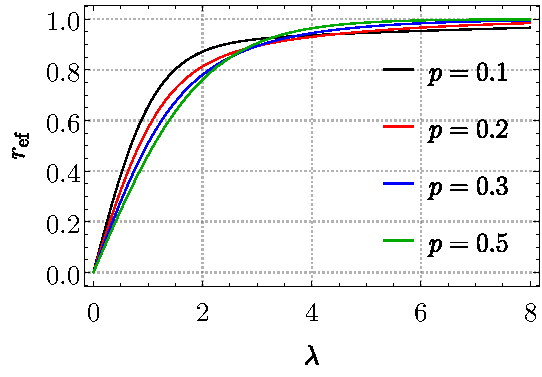
\includegraphics[width=0.5\linewidth]{chapter3/figures/r(lambda).pdf}
    \caption{$r_{\ef}$ como función de $\lambda$ para diferentes valores de $p_{1}$ en el caso en que $n=2$.}
    \label{fig:r(lambda)}
\end{figure}

\subsection{Otra expresión del estado de máxima entropía}

\acnote{Al final nunca usé esto, ¿se queda?}

La ecuación (\ref{eq:MaxEntSeparable}) sugiere que el estado de máxima entropía puede expresarse como producto tensorial de potencias de un mismo estado. En efecto, dado un real $q$ y una matriz cuadrada $A$, la potenciación $A^{q}$ puede escribirse como $e^{q \ln A}$. Como las matrices $e^{\sum_{i}\lambda_{i}\pauli{i}}$ son positivas semidefinidas, su logaritmo es único en el caso de no ser degenerado, y en caso de degeneración, basta con tomar la rama principal \cite{log1,Davalos2019}. Entonces,
\begin{equation}
    \varrho_{\max}=\Motimes_{j=1}^{n}\frac{1}{Z_{j}}e^{p_{j}\sum_{k}\lambda_{k}\pauli{k}}=\Motimes_{j=1}^{n}\frac{1}{Z_{j}}\qty(e^{\sum_{k}\lambda_{k}\pauli{k}})^{p_{j}}.\nonumber
\end{equation}
En virtud de (\ref*{ap:PauliRealExp}), se cumple que
\begin{align}
  \varrho_{\max}=&\Motimes_{j=1}^{n}\frac{\qty(\cosh{\lambda}(\Id+\tanh{\lambda}(\paulivec{r_{\rho}})))^{p_{j}}}{\Tr[\qty(\cosh{\lambda}(\Id+\tanh{\lambda}(\paulivec{r_{\rho}})))^{p_{j}}]}\nonumber\\
  =&\Motimes_{j=1}^{n}\frac{\qty(\Id+\tanh{\lambda}(\paulivec{r_{\rho}}))^{p_{j}}}{\Tr[\qty(\Id+\tanh{\lambda}(\paulivec{r_{\rho}}))^{p_{j}}]}.\nonumber
\end{align}
Definimos
\begin{equation}\label{eq:Xi}
  \Xi_{\max}=\frac{1}{2}(\Id+\tanh{\lambda}(\paulivec{r_{\rho}})),
\end{equation}
de tal manera que 
\begin{equation}\label{eq:MaxEntSeparablePower}
  \varrho_{\max}=\Motimes_{j=1}^{n}\frac{(\Xi_{\max})^{p_{j}}}{\Tr[ (\Xi_{\max})^{p_{j}}]}.
\end{equation}

\subsection{La asignación de máxima entropía}

El estado de máxima entropía nos otorga una herramienta de asignación para los estados efectivos. Después de todo, requerimos de una asignación razonable que pueda ser propagada según la dinámica microscópica conocida. Sea $\rho_{\ef}\in\densityspace{2}$ un estado efectivo, entonces definimos a la aplicación de asignación de máxima entropía como
\begin{equation}\label{eq:MaxEntAss}
    \begin{gathered}
        \mcA_{\mcC}^{\max}:\densityspace{2}\rightarrow\densityspace{2^{n}}\nonumber\\
        \rho_{\ef} \mapsto \Motimes_{j=1}^{n}\frac{1}{Z_{j}}\text{exp}\qty(p_{j}\sum_{k=1}^{3}\lambda_{k}\sigma_{k}).
    \end{gathered}
\end{equation}
donde la dependencia de la asignación en el modelo de grano grueso se indica mediante un subíndice, $\mcC$. Nótese que según los valores que puedan tomar las diferentes probabilidades $p_{j}$, el estado asignado tendrá diferentes propiedades. Nos concentramos en dos casos particulares. El primero corresponde a $p_{1}=1$. En este caso se eliminan los términos de error, y el estado de máxima entropía es simplemente
\begin{equation}\label{eq:PreferentialAss}
    \varrho_{\max}=\rho_{\ef}\otimes\Id^{2^{n-1}},
\end{equation}
Nótese que la aplicación de asignación se vuelve lineal si no hay error de medición. Esto debe verse como un caso límite. Este trabajo estudiará $p_{1}\rightarrow 1$ como el escenario en el que la probabilidad de detectar la partícula equivocada es pequeña. De acuerdo con esto, se le llamará  \textit{regimen de partícula preferencial}.

Ahora, si por otro lado, $p_{j}=\frac{1}{n}\forall j$, entonces el estado de máxima entropía es
\begin{equation}
    \varrho_{\max}=\qty[\frac{1}{Z}\text{exp}\qty(\frac{1}{n}\sum_{k=1}^{3}\lambda_{k}\sigma_{k})]^{\otimes n}=(\rho')^{\otimes n}.\nonumber
\end{equation}
Si se pasa este estado por la aplicación de grano grueso correspondiente el resultado es 
\begin{equation}
    \mcC[\varrho_{\max}]=\sum_{j=1}^{n}\frac{1}{n}\rho'=\rho',\nonumber
\end{equation}
de  lo que se concluye que
\begin{equation*}
    \rho'=\rho_{\ef},
\end{equation*}
y que por lo tanto el estado asignado es simplemente
\begin{equation}\label{eq:BoltzmannAss}
    \mcA_{\mcC}^{\max}(\rho_{\ef})=\rho_{\ef}^{\otimes n}.
\end{equation}
Así, si $p_{j}=\frac{1}{n}\forall j$, la asignación de máxima entropía resulta en un estado factorizable de $n$ partículas idénticas. A este caso se le llamará \textit{régimen imparcial}.



Ahora supóngase que $\varrho$ es un estado microscópico compatible con un estado efectivo puro $\rho_{\ef}=\dyad{\psi}$, y que $p_{j}\neq 0\,\forall\,j$. Entonces, por (\ref{eq:MaxEntSeparable}) se cumple que
\begin{equation}
    \rho_{ef}=\sum_{k=1}^{n}p_{k}\varrho_{k},\nonumber
\end{equation}
donde $\varrho_{k}\in\densityspace{2}$ es la $k$-ésima traza parcial de $\varrho$. Como se mencionó en la sección \ref{subsec:ch2_purity}, un estado puro es un punto extremo del conjunto de estados, así que la ecuación anterior solo se puede cumplir si $\varrho_{k}=\dyad{\psi}\,\forall\,k$.  Si cada traza parcial de $\varrho$ es igual al estado puro $\rho_{\ef}$ se sigue que
\begin{equation}\label{eq:PureEffectiveState}
    \varrho=\left(\dyad{\psi}\right)^{\otimes n}.
\end{equation}
Nótese que para obtener (\ref{eq:PureEffectiveState}) no se hizo ninguna suposición sobre la aplicación de asignación. Lo que se acaba de demostrar es que, dado que todas las trazas parciales participen en la aplicación de grano grueso, el único estado microscópico compatible con un estado efectivo puro es el $n$-producto de dicho estado. El estado (\ref{eq:PureEffectiveState}) es un estado coherente de espín~\cite{klimovbook}~\footnote{Los estados coherentes de $n$ espines $1/2$ consisten en estados puros donde todas las partículas están ``alineadas'' en la misma dirección en la esfera de Bloch. Es decir, simplemente se tiene que $\ket{\psi_\text{coh}}=\ket\psi^{\otimes n}$, en virtud de que estos estados saturan la relaciones de incertidumbre de espín.}.

\section{Construcción de la dinámica}\label{sec:ch2dycon}

Ahora que hemos establecido que usaremos como modelo de grano grueso uno que incluye tanto problemas de resolución como errores de permutación, y que hemos contruído nuestra aplicación de asignación a través del Principio de Máxima Entropía, podemos preguntarnos sobre la evolución del sistema efectivo, la ``dinámica gruesa'', denotada como $\Gamma_t$. La dinámica efectiva es un mapa dinámico que corresponde a la evolución observada por un experimentalista. Dado un estado efectivo inicial $\rho_{\ef}(0)$,
\begin{gather}
\Gamma_{t}:\mcS(\hilbert_2)\rightarrow \mcS(\hilbert_2)\nonumber\\
\rho_{\ef}(0) \mapsto \rho_{\ef}(t)\rlap{.}\nonumber
\end{gather}
Debido que asumimos que el estado que se propaga debido a la evolución subyacente es justamente el estado de máxima entropía, a la dinámica gruesa la definimos como la composición
\begin{equation}
\Gamma_t:=\mcC \circ \mcV_t \circ \mcA_\mcC.\nonumber
\end{equation}
Donde $\mcA_\mcC$ denota a la aplicación que asigna un estado microscópico $\varrho$ al estado efectivo $\rho_{\ef}$. A la aplicación de asignación desarrollada previamente la denotaremos por medio de $\mcA_{\mcC}^{\max}$. El siguiente diagrama ilustra la ecuación anterior,
\[\begin{tikzcd}[arrows={<-|}]
    \rho_{\ef}(0)  & \rho_{\ef}(t) \arrow{l}{\Gamma_{t}} \arrow{d}{\mcC}\\
\varrho(0) \arrow{u}{\mcA_{\mcC}^{\max}} & \varrho(t). \arrow{l}{\mcV_{t}}
\end{tikzcd}
\]
En el siguiente capítulo se analizarán dinámicas efectivas generadas por diferentes dinámicas subyacentes. Si se asume que el sistema conformado por las partículas es cerrado, entonces la evolución $\mcV_{t}$ será unitaria, generada por un hamiltoniano $H$. Algunos ejemplos de dinámicas subyacentes no unitarias son los canales de ruido usuales, como el canal de despolarización, el canal de amortiguamiento de amplitud, o el canal de amortiguamiento de fase.

Nótese que, a diferencia de los mapas dinámicos usualmente estudiados en teoría de sistemas cuánticos abiertos, la dinámica efectiva $\Gamma_{t}$ no tiene por qué ser lineal (sí debe, por supuesto, mandar estados en estados), debido a que uno de los elementos de la composición que la originan no es lineal: la aplicación de asignación. El estudio de las particularidades de algunas de estas dinámicas efectivas es el foco de este trabajo.

Reconociendo que la asignación de máxima entropía no es la única asignación compatible con un conjunto de aplicación de grano grueso y estado inicial efectivo, ¿es justificable usar al estado de máxima entropía? Previamente demostramos que en nuestro caso particular, este resulta ser separable, y aunque en el caso estacionario esto no afecta, las correlaciones, que se anulan en esta asignación, sí afectan la forma en que un sistema evoluciona.

Algo que queda en claro de esto es que el estado de máxima entropía es completamente dependiente de los observables que se usen en su construcción. Después de todo, la maximización de la entropía se restringe de acuerdo a las observaciones experimentales, así que estados de máxima entropía que cumplan un conjunto particular de restricciones no tienen por qué (y probablemente no lo harán) satisfacer un conjunto diferente de restricciones, un conjunto mediante el cual se construiría un estado de máxima entropía diferente. Esto tiene la siguiente consecuencia: el estado de máxima entropía compatible con un estado evolucionado a través de una dinámica efectiva obtenida de un estado de máxima entropía compatible con un estado efectivo inicial, no tiene por qué ser igual al estado de máxima entropía inicial evolucionado. Esto es, no tiene por que cumplirse que
\begin{equation}
    (\mcU_{t}\circ\mcA_\mcC)(\rho) = (\mcA_\mcC\circ\mcC \circ \mcU_t \circ \mcA_\mcC)(\rho).\nonumber
\end{equation}
Y la razón de esto es que
\begin{equation}
    \mcA_\mcC\neq\mcC^{-1}.\nonumber
\end{equation}


\newpage
